\documentclass[11pt,a4paper]{article}
\usepackage[margin=0.85in]{geometry}
\usepackage{amsmath,amssymb,amsthm}
\usepackage{tikz}
\usetikzlibrary{arrows.meta,positioning,shapes.geometric,fit,backgrounds,calc,decorations.pathmorphing}
\usepackage{algorithm}
\usepackage{algpseudocode}
\usepackage{booktabs}
\usepackage{hyperref}
\usepackage{xcolor}
\usepackage{enumitem}

\definecolor{ethblue}{RGB}{0,105,180}
\definecolor{ethgreen}{RGB}{98,164,63}
\definecolor{ethred}{RGB}{183,53,45}

\title{\textbf{Adaptive Majorana-Neural Propagation for Non-Hermitian Quantum Many-Body Dynamics}}
\author{H M Shujaat Zaheer\\
\small Research Proposal for PhD Position\\
\small Quantum AI Lab, ETH Z\"urich\\
\small Supervisor: Prof. Juan Carrasquilla}
\date{January 2026}

\begin{document}
\maketitle

\begin{abstract}
We propose the \textbf{Adaptive Majorana-Neural Propagation (AMNP)} framework, unifying autoregressive neural quantum states with Majorana string truncation for simulating \textbf{non-Hermitian} strongly correlated fermionic systems. The framework addresses three fundamental gaps in current methods: (1) the optimizer incompatibility between Stochastic Reconfiguration and RNN wave functions, (2) Majorana truncation rules breaking for non-Fock variational states, and (3) restriction of fermionic neural Gibbs states to Hermitian closed systems. We introduce three novel algorithmic contributions: \textbf{Geometry-Aware Stochastic Reconfiguration (GASR)}, \textbf{Non-Hermitian Trotter-Consistent Truncation (NHTCT)}, and \textbf{Thermofield-Extended Neural Gibbs States (TENGS)}. These innovations enable accurate simulation of dissipative Fermi-Hubbard dynamics, non-Hermitian kagome lattices, and open-system quantum transport beyond existing classical methods.
\end{abstract}

\section{Introduction and Motivation}

Neural quantum states (NQS) have emerged as powerful variational representations for quantum many-body systems~[1,2]. Recent advances demonstrate that recurrent neural network (RNN) wave functions achieve state-of-the-art accuracy for frustrated spin systems~[3], while Majorana string propagation enables efficient 2D fermionic dynamics simulation~[4]. Simultaneously, fermionic neural Gibbs states capture finite-temperature correlations in doped Fermi-Hubbard models~[5]. However, critical limitations prevent these methods from addressing \textbf{non-Hermitian} quantum systems—central to dissipative dynamics, quantum transport, and open quantum systems.

\begin{figure}[h]
\centering
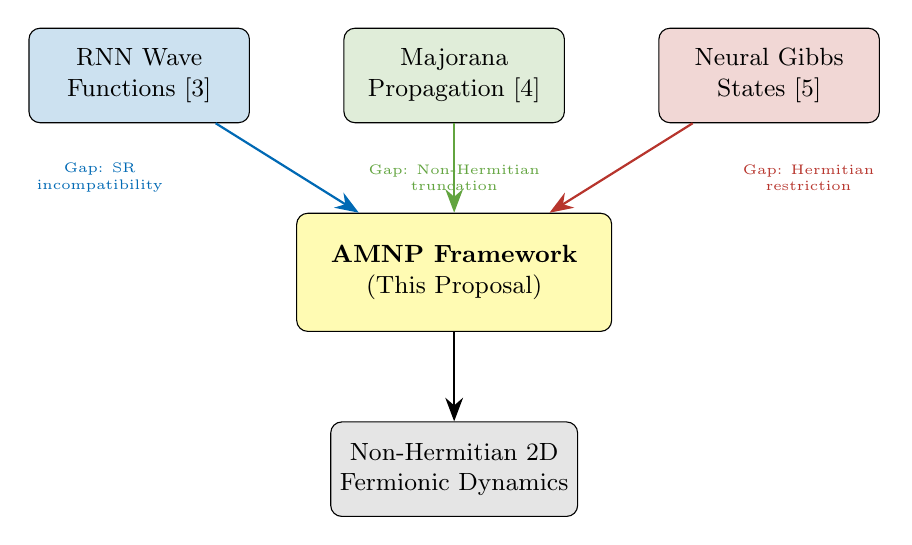
\begin{tikzpicture}[
    box/.style={draw, rounded corners, minimum width=2.8cm, minimum height=1.2cm, align=center, font=\small},
    arrow/.style={-{Stealth[length=3mm]}, thick}
]
% Three input methods
\node[box, fill=ethblue!20] (rnn) at (0,3) {RNN Wave\\Functions~[3]};
\node[box, fill=ethgreen!20] (maj) at (4,3) {Majorana\\Propagation~[4]};
\node[box, fill=ethred!20] (gibbs) at (8,3) {Neural Gibbs\\States~[5]};

% Central unifying framework
\node[box, fill=yellow!30, minimum width=4cm, minimum height=1.5cm] (amnp) at (4,0.5) {\textbf{AMNP Framework}\\(This Proposal)};

% Output capabilities
\node[box, fill=gray!20] (output) at (4,-2) {Non-Hermitian 2D\\Fermionic Dynamics};

% Arrows
\draw[arrow, ethblue] (rnn) -- (amnp);
\draw[arrow, ethgreen] (maj) -- (amnp);
\draw[arrow, ethred] (gibbs) -- (amnp);
\draw[arrow, thick, black] (amnp) -- (output);

% Gap labels
\node[font=\tiny, align=center, text=ethblue] at (-0.5,1.7) {Gap: SR\\incompatibility};
\node[font=\tiny, align=center, text=ethgreen] at (4,1.7) {Gap: Non-Hermitian\\truncation};
\node[font=\tiny, align=center, text=ethred] at (8.5,1.7) {Gap: Hermitian\\restriction};

\end{tikzpicture}
\caption{Research landscape: AMNP unifies three recent advances while addressing their identified limitations.}
\label{fig:landscape}
\end{figure}

\section{Problem Statement and Identified Gaps}

\subsection{Gap 1: Optimizer Incompatibility in Autoregressive NQS}
Recent work on kagome lattice Rydberg arrays~[3] demonstrates that ``\textit{Stochastic Reconfiguration is not as effective as Adam optimizer when applied to RNN wave functions}.'' The quantum geometric tensor $S_{kk'} = \langle \Delta O_k^* \Delta O_{k'} \rangle$ becomes ill-conditioned for autoregressive architectures due to sequential sampling correlations, causing convergence instabilities.

\subsection{Gap 2: Majorana Truncation for Non-Hermitian Systems}
The Majorana string propagation framework~[4] introduces Trotter-consistent truncation: discard strings with unpaired Majoranas $w_s(v) > S$. However, this assumes \textbf{Fock-state initial conditions}—the overlap condition $\langle n_1 \cdots n_N | \mu(v) | n_1 \cdots n_N \rangle \neq 0$ requires $v_{2k-1} = v_{2k}$. For variational initial states or non-Hermitian Hamiltonians with complex eigenvalues, these truncation rules fail to preserve Trotter accuracy.

\subsection{Gap 3: Hermitian Restriction in Neural Thermal States}
The fermionic neural Gibbs states~[5] achieve accurate thermal energies via thermofield-double purification with work-operator evolution. However, the framework assumes Hermitian Hamiltonians: $W = \hat{H} \otimes \tilde{I} - \frac{\beta_0}{\beta} \hat{I} \otimes \tilde{H}_0$. Extensions to ``\textit{real-time dynamics and non-Hermitian steady states require new theoretical frameworks}''~[5].

\section{Proposed Innovations}

\subsection{Geometry-Aware Stochastic Reconfiguration (GASR)}

We propose an adaptive optimizer interpolating between curvature-aware (SR) and first-order (Adam) updates based on gradient signal-to-noise ratio:
\begin{equation}
G_{\text{GASR}} = (1-\alpha)S + \alpha J^T J + \lambda I
\end{equation}
where $S$ is the quantum geometric tensor, $J$ is the Jacobian of log-amplitudes, and $\alpha = \sigma(\log \rho - \tau)$ adapts based on effective signal-to-noise $\rho = \|g\|^2 / \text{Var}[g]$.

\begin{algorithm}[h]
\caption{Geometry-Aware Stochastic Reconfiguration (GASR)}
\begin{algorithmic}[1]
\Require Ansatz $|\psi_\theta\rangle$, learning rate $\eta$, threshold $\tau$
\State Sample configurations $\{x_i\}_{i=1}^{N_s}$ from $|\psi_\theta|^2$
\State Compute local energies $E_{\text{loc}}(x_i) = \langle x_i | \hat{H} | \psi_\theta \rangle / \psi_\theta(x_i)$
\State Compute gradient $g_k = \langle O_k^* (E_{\text{loc}} - \langle E \rangle) \rangle$
\State Estimate SNR: $\rho \gets \|g\|^2 / \text{Var}[g]$
\State Adaptive interpolation: $\alpha \gets \sigma(\log \rho - \tau)$
\State Construct $G_{\text{GASR}} = (1-\alpha)S + \alpha J^T J + \lambda I$
\State Update: $\theta \gets \theta - \eta \cdot G_{\text{GASR}}^{-1} g$
\State \Return Updated parameters $\theta$
\end{algorithmic}
\end{algorithm}

\subsection{Non-Hermitian Trotter-Consistent Truncation (NHTCT)}

For non-Hermitian Hamiltonians $H = H_{\text{Herm}} + i\Gamma$, complex eigenvalues cause exponential growth/decay. We introduce \textbf{decay-bounded truncation}:
\begin{equation}
\text{Truncate if: } w_s(v) > S \text{ OR } |\text{Im}[\lambda_v]| > \Gamma_{\max}
\end{equation}
where $\Gamma_{\max} = -\frac{1}{\delta\tau}\ln(\epsilon_{\text{Trotter}})$ ensures truncation errors remain within Trotter accuracy.

\begin{figure}[h]
\centering
\begin{tikzpicture}[scale=0.9]
% Complex plane
\draw[-{Stealth}] (-3,0) -- (3,0) node[right] {Re$[\lambda]$};
\draw[-{Stealth}] (0,-2.5) -- (0,2.5) node[above] {Im$[\lambda]$};

% Truncation region
\fill[ethgreen!20] (-2.5,-1.5) rectangle (2.5,1.5);
\draw[ethgreen, thick, dashed] (-2.5,-1.5) -- (2.5,-1.5);
\draw[ethgreen, thick, dashed] (-2.5,1.5) -- (2.5,1.5);

% Eigenvalues
\foreach \x/\y in {-1.8/0.5, -0.5/1.2, 0.8/-0.8, 1.5/0.3, -1.2/-1.8, 2.1/1.9}{
    \ifnum\y>150 \fill[ethred] (\x,\y) circle (3pt);
    \else \ifnum\y<-150 \fill[ethred] (\x,\y) circle (3pt);
    \else \fill[ethblue] (\x,\y) circle (3pt);
    \fi\fi
}
\fill[ethred] (-1.2,-1.8) circle (3pt);
\fill[ethred] (2.1,1.9) circle (3pt);

% Labels
\node[font=\small] at (0,2.0) {$\Gamma_{\max}$};
\node[font=\small] at (0,-2.0) {$-\Gamma_{\max}$};
\node[font=\small, ethgreen] at (3.5,0) {\textbf{Keep}};
\node[font=\small, ethred] at (3.5,2) {\textbf{Truncate}};

\end{tikzpicture}
\caption{NHTCT eigenvalue truncation in complex plane. Strings with eigenvalues outside $[-\Gamma_{\max}, \Gamma_{\max}]$ are pruned.}
\label{fig:nhtct}
\end{figure}

\subsection{Thermofield-Extended Neural Gibbs States (TENGS)}

We extend the work operator to non-Hermitian systems:
\begin{equation}
W_{\text{NH}} = \hat{H} \otimes \tilde{I} - \frac{\beta_0}{\beta} \hat{I} \otimes \tilde{H}_0 + i\Gamma \otimes \tilde{I}
\end{equation}
The dissipator $\Gamma$ captures particle loss, gain, or dephasing. Imaginary-time evolution via Taylor-root expansion projected ITE (tre-pITE)~[5] generalizes to complex-time contours.

\begin{figure}[h]
\centering
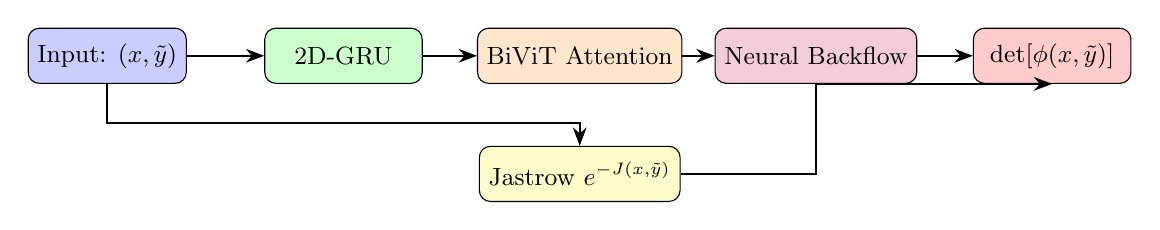
\begin{tikzpicture}[
    layer/.style={draw, rounded corners, minimum width=2cm, minimum height=0.7cm, font=\small},
    arrow/.style={-{Stealth}, thick}
]
% Input layer
\node[layer, fill=blue!20] (input) at (0,0) {Input: $(x, \tilde{y})$};

% 2D-GRU layer
\node[layer, fill=green!20] (gru) at (3,0) {2D-GRU};

% Attention layer
\node[layer, fill=orange!20] (attn) at (6,0) {BiViT Attention};

% Backflow
\node[layer, fill=purple!20] (backflow) at (9,0) {Neural Backflow};

% Output
\node[layer, fill=red!20] (output) at (12,0) {$\det[\phi(x,\tilde{y})]$};

% Arrows
\draw[arrow] (input) -- (gru);
\draw[arrow] (gru) -- (attn);
\draw[arrow] (attn) -- (backflow);
\draw[arrow] (backflow) -- (output);

% Jastrow branch
\node[layer, fill=yellow!20] (jastrow) at (6,-1.5) {Jastrow $e^{-J(x,\tilde{y})}$};
\draw[arrow] (input.south) -- ++(0,-0.5) -| (jastrow);
\draw[arrow] (jastrow) -- ++(3,0) |- (output.south);

\end{tikzpicture}
\caption{TENGS neural architecture: BiViT attention captures inter-species correlations between physical and auxiliary fermions.}
\label{fig:tengs}
\end{figure}

\begin{algorithm}[h]
\caption{TENGS Evolution for Non-Hermitian Systems}
\begin{algorithmic}[1]
\Require Mean-field state $|\Psi_0(\beta_0)\rangle$, target $\beta$, dissipator $\Gamma$
\State Initialize pair orbitals $\phi \gets \phi_0$ from mean-field
\State Construct work operator $W_{\text{NH}} = \hat{H} \otimes \tilde{I} - \frac{\beta_0}{\beta} \hat{I} \otimes \tilde{H}_0 + i\Gamma \otimes \tilde{I}$
\For{$\tau = 0$ to $\beta/2$ by $\delta\tau$}
    \State Sample $(x, \tilde{y}) \sim |\Psi_\theta|^2$
    \State Compute fidelity gradient via tre-pITE~[5]
    \State Update $\theta$ using GASR optimizer
\EndFor
\State \Return Thermal state $|\Psi(\beta)\rangle$
\end{algorithmic}
\end{algorithm}

\section{Target Systems and Validation}

\begin{table}[h]
\centering
\caption{Target systems and comparison with existing methods}
\begin{tabular}{lccc}
\toprule
\textbf{System} & \textbf{AMNP} & \textbf{MPS/fPEPS} & \textbf{QMC} \\
\midrule
Dissipative Fermi-Hubbard & \checkmark & Limited & Sign problem \\
Non-Hermitian kagome & \checkmark & $\times$ & $\times$ \\
Open-system transport & \checkmark & 1D only & $\times$ \\
Finite-T non-Hermitian & \checkmark & $\times$ & $\times$ \\
\bottomrule
\end{tabular}
\end{table}

\textbf{Validation Protocol:} Following variational benchmarks~[1], we report v-scores comparing energy accuracy against exact diagonalization (small systems) and quantum Monte Carlo (where applicable). Correlation functions $C_{ss}(\mathbf{d})$ and structure factors $S(\mathbf{q})$ verify physical consistency.

\section{Expected Contributions}

\begin{enumerate}[leftmargin=*]
\item \textbf{Theoretical:} First framework unifying NQS with non-Hermitian dynamics; complexity bounds for NHTCT; convergence analysis of GASR optimizer.
\item \textbf{Algorithmic:} Three novel algorithms (GASR, NHTCT, TENGS) with open-source NetKet implementation.
\item \textbf{Practical:} Benchmarks for dissipative 2D fermionic systems beyond tensor network capabilities; protocols for quantum simulator validation.
\end{enumerate}

\section{Conclusion}

The AMNP framework addresses fundamental limitations in current neural quantum state methods by introducing geometry-aware optimization, non-Hermitian truncation schemes, and thermofield extensions to dissipative systems. This research will advance our capability to simulate strongly correlated fermionic dynamics in regimes inaccessible to existing classical methods, with direct applications to quantum materials, superconductivity, and quantum device physics.

\section*{References}
\footnotesize
\begin{enumerate}[label={[\arabic*]}, leftmargin=*, itemsep=0pt]
\item D. Wu \textit{et al.}, ``Variational benchmarks for quantum many-body problems,'' \textit{Science}, vol. 386, pp. 296--301, 2024.
\item G. Carleo and M. Troyer, ``Solving the quantum many-body problem with artificial neural networks,'' \textit{Science}, vol. 355, pp. 602--606, 2017.
\item M. Hibat-Allah \textit{et al.}, ``Recurrent neural network wave functions for Rydberg atom arrays on kagome lattice,'' \textit{Commun. Phys.}, vol. 8, p. 308, 2025.
\item M. D'Anna, J. Nys, and J. Carrasquilla, ``Majorana string simulation of nonequilibrium dynamics in two-dimensional lattice fermion systems,'' \textit{arXiv:2511.02809}, 2025.
\item J. Nys and J. Carrasquilla, ``Fermionic neural Gibbs states,'' \textit{arXiv:2512.04663}, 2025.
\item M. S. Moss \textit{et al.}, ``Leveraging recurrence in neural network wavefunctions for large-scale simulations of Heisenberg antiferromagnets,'' \textit{Phys. Rev. B}, vol. 112, p. 134450, 2025.
\item Y. Zhang, J. Carrasquilla, and Y. B. Kim, ``Observation of a non-Hermitian supersonic mode on a trapped-ion quantum computer,'' \textit{Nat. Commun.}, vol. 16, p. 3286, 2025.
\item M. Medvidovi\'c \textit{et al.}, ``Adiabatic transport of neural network quantum states,'' \textit{arXiv:2510.15030}, 2025.
\item B. Barton \textit{et al.}, ``Interpretable scaling behavior in sparse subnetwork representations of quantum states,'' \textit{arXiv:2505.22734}, 2025.
\item A. D. King \textit{et al.}, ``Beyond-classical computation in quantum simulation,'' \textit{Science}, vol. 388, pp. 199--204, 2025.
\end{enumerate}

\end{document}
